%=========================================================================
% (c) Michal Bidlo, Bohuslav Křena, 2008

% Start of text
\chapter{Introduction}

Focus of this thesis is a performance optimization of Red Hat's BeakerLib library, particularly its Journal feature. <expand>
\\
\\
The thesis is structured in a following way: chapter \ref{relevant_projects} introduces projects relevant to BeakerLib and its testing environment. Chapter \ref{beakerlib_chapter} explains more in-depth how BeakerLib works, with focus on its Journal feature and analysis of its performance. In the chapter \ref{solutions} possible optimizations are discussed and chapter \ref{implementations} focuses on implementation of proposed solutions. The chapter \ref{performance} then describes how was performance measured and in what environment. <expand>

\chapter{Relevant projects}
\label{relevant_projects}

This this chapter describes BeakerLib and projects relevant to it. Nejprve je popsana knihovna jako takova, nasledujici sekce se venuje Beaker coz je system from which BeakrLib originally  a posledni sekce popisuje test harnessy

\section{BeakerLib}

BeakerLib is a Linux shell-level integration testing library, providing convenience functions which simplify writing, running and analysis of integration and blackbox tests. \cite{beakerlib_wiki}
It is developed and maintained by Red Hat and operates under GNU General Public License.
Main features of BeakerLib include:
\begin{itemize}
\item Journal - uniform logging mechanism (logs and results saved in flexible XML format, easy to compare results and generate reports)
\item Phases - logical grouping of test actions, clear separation of setup / test / cleanup
\item Asserts - common checks affecting the overall results of individual phases (checking for exit codes, file existence and content...)
\item Helpers - convenience functions for common operations such as managing system services, backup and restore of files and more
\end{itemize}


This thesis focuses on BeakerLib Journal and problem it causes with long tests. ??? Which will be described in chapter ...


\section{Beaker}

Beaker\cite{beaker_doc} is a full stack software and hardware integration testing system, with the ability to manage a globally distributed network of test labs.  It is Red Hat community project under GNU General Public License version 2.

Main functionality includes management of hardware inventory, on which Beaker can install wide variety  of operating systems from Red Hat Linux family. Another notable part  is Task library which contains rpm packages of individual tests which can be run on provided machines. 
Users then can specify which hardware they require with which OS and tests they want to run on it through either command-line tools or web interface both of which are part of Beaker install package. If Beaker meets given criteria in its inventory it installs Test harness to which it gives list of tests to be run.  After Test Harness finishes running the tests, results are sent back to Beaker where they are stored for specified period of time. 

\subsection{beaker-wizard}
Part of Beaker package. Interactive command-line tool which automates creation of BeakerLib tests. Using predefined or user-defined templates it creates all files that are needed to run BeakerLib test. 
???  Common use cases

\section{Test Harness}
Test harness is a software framework that automates test execution. It contains tests to be run, executes them and reports results. <expand>

Beaker’s harnesses prepare provided machine for BeakerLib by setting environmental variables to proper values, and then running the tests.

\subsection{Beah harness}
Beah \cite{beah_doc} is a default Beaker harness . <expand> 

\subsection{Restraint harness}
Restraint \cite{restraint_doc} is an alternative Beaker harness which can, unlike Beah, run with Beaker or standalone without it. <expand>

\section{Projects' relation}
Relation between Beaker, Harness and BeakerLib is shown in figure \ref{fig:beaker_relation}. In this example user submits Beaker job containing three tests and hardware/software requirements for a machine the tests should run on. After Beaker reserves it, it installs Harness which successively executes each test and uploads their results back to Beaker when user can access them.

\begin{figure}[h!]
  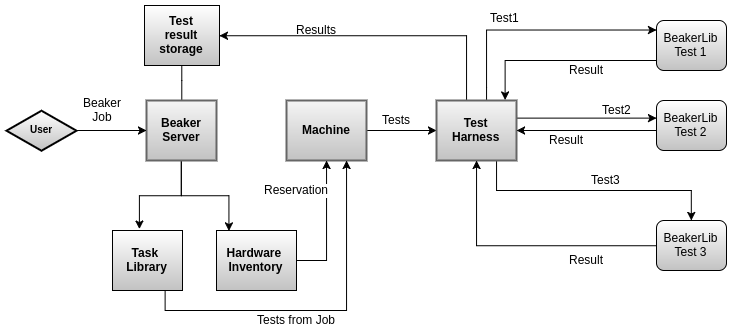
\includegraphics[width=\linewidth]{beaker_relations.png}
  \caption{Beaker relation to BeakerLib}
  \label{fig:beaker_relation}
\end{figure}

\chapter{BeakerLib}
\label{beakerlib_chapter}

This chapter takes a closer look on inner workings of BeakerLib, with focus on Journal feature and performance issues it suffers from.

\section{Important functions}
As stated earlier BeakerLib is shell-level library with functions that make writing and running tests easier as well as examining their results.
BeakerLib adds testing functions to \texttt{shell} functionality, so user can combine normal \texttt{shell} commands and constructions with helping functions which can make writing tests and examining their results easier. There is close to 80 of these functions (also known as \textbf{rlCommands}), description of most used ones follows:
\begin{itemize}
\item \textbf{rlRun} - First argument of this function is any shell command, which is executed by rlRun. Second is an expected exit code of first argument, it can contain one or more codes. Third argument is a comment. BeakerLib logs \texttt{FAIL} or \texttt{PASS} if expected exit code differs or not from actual one respectively along with comment. This is most used and important function.
\item \textbf{rlPass} - Manual assertion and logging of \texttt{PASS}. Useful when in combination with if statement which user doesn't want to appear in logs but still wants to log its result. Reciprocal function \textbf{rlFail} exists as well.
\item \textbf{rlAssertExists} - Asserts whether file given as a first argument exists.
\item \textbf{rlAssertGrep} - Function logs \texttt{PASS} when pattern given as first argument matches in a file which is given a second argument. Optional flags are passed to \texttt{grep} and behave the same way.
\item \textbf{rlAssertRpm} - Function asserts \texttt{PASS} when package given as first argument is installed.  Optional arguments allow specifying particular version, release or arch of the package.
\item \textbf{rlAssertDiffer} - Asserts whether two files given as argument differ in their content. 
\item \textbf{rlJournalStart} - This function is used at the start of each test. It is essential for proper run of the test as it initializes BeakerLib's  outputs, which described later in this chapter. Reciprocal function \textbf{rlJournalEnd} must be called at the end of the test.
\item \textbf{rlPhaseStart} - This function starts user-defined phase. Function takes two arguments, first one is a type of phase, second one is a name. Phase must be ended by calling \textbf{rlPhaseEnd}. Phases are more closely explained in the next section.
\end{itemize}

\section{Phases}
BeakerLib divides tests into logical groups called Phases. There are three predefined types of phases:
\begin{itemize}
\item Setup - Preparing conditions for the test (such as creating temporary files, starting needed system services and so on), started by calling \textbf{rlPhaseStartSetup}.
\item Test - Main phase for testing, started by calling \textbf{rlPhaseStartTest}.
\item Cleanup - Reverting changes made by the test, started by calling \mbox{\textbf{rlPhaseStartCleanup}}.
\end{itemize}

Apart from predefined Phases, user can also define own phases by calling \textbf{rlJournalStart} function. First argument of the function is a one of two types phase can have:

\begin{itemize}
\item WARN - if any \textbf{rlCommand} in phase of this type fails, whole phase will result in Warning state.
\item FAIL - similar to previous type however this time resulting in Failed state.
\end{itemize}

Basic phases Setup and Cleanup are WARN type, Test phase is a FAIL type.

The result of the whole test is the same as the worst result of any phase in the order: Failed, Warning, Passed.
Asserts made outside of phases will automatically fail.

This division helps with examining the result of test as it shows which phase, if any, causes fail in BeakerLib's output. 
example test \ref{lst:test_example} shows how basic BeakerLib test looks.
\\
\begin{lstlisting}[style=beakerlib_bash,caption={BeakerLib basic test example},label={lst:test_example}]
# Include Beaker environment
. /usr/bin/rhts-environment.sh || exit 1
. /usr/share/beakerlib/beakerlib.sh || exit 1
# Start of Journal
rlJournalStart
    # Start of Setup Phase, creating temp directory where test will take place 
    rlPhaseStartSetup
        rlAssertRpm $PACKAGE
        rlRun "TmpDir=\$(mktemp -d)" 0 "Creating tmp directory"
        rlRun "pushd $TmpDir"
    rlPhaseEnd
   # Start of Test Phase, testing touch and ls commands
    rlPhaseStartTest
        rlRun "touch foo" 0 "Creating the foo test file"
        rlAssertExists "foo"
        rlRun "ls -l foo" 0 "Listing the foo test file"
    rlPhaseEnd
   # Statr of Cleanup phase, temp directory is deleted
    rlPhaseStartCleanup
        rlRun "popd"
        rlRun "rm -r $TmpDir" 0 "Removing tmp directory"
    rlPhaseEnd
rlJournalPrint
rlJournalEnd
\end{lstlisting}

\section{BeakerLib's output}
BeakerLib produces three kinds of outputs, two file formats and a console one which are described in this section. Files are saved into a directory created for each individual test. If the test is run locally, temporary directory is created on system with \texttt{mktepm} command. If run on Beaker unique \textbf{TESTID} is generated for each test. This \textbf{TESTID} serves as a name for test directory as well as identifier which Beaker later uses when connecting test results with correct test.

\subsection{journal.txt}
\textit{journal.txt} is a plain text file with human readable record of test's progress. After end of each phase, copy of the file is sent to Beaker for storage. Snippet of \textit{journal.txt} generated by Example test \ref{lst:test_example} is shown in \ref{lst:journaltxt_example}.


\begin{lstlisting}[style=txt,caption={Example of journal.txt},label={lst:journaltxt_example}]
::::::::::::::::::::::::::::::::::::::::::::::::::::::::::::::::::::::::::::::::
:: [   LOG    ] :: Setup
::::::::::::::::::::::::::::::::::::::::::::::::::::::::::::::::::::::::::::::::

:: [   PASS   ] :: Checking for the presence of bash rpm
:: [   LOG    ] :: Package versions:
:: [   LOG    ] ::   bash-4.3.43-4.fc25.x86_64
:: [   PASS   ] :: Creating tmp directory (Expected 0, got 0)
:: [   PASS   ] :: Command 'pushd /tmp/tmp.oawaORcDNI' (Expected 0, got 0)
:: [   LOG    ] :: Duration: 1s
:: [   LOG    ] :: Assertions: 3 good, 0 bad
:: [   PASS   ] :: RESULT: Setup

::::::::::::::::::::::::::::::::::::::::::::::::::::::::::::::::::::::::::::::::
:: [   LOG    ] :: Test
::::::::::::::::::::::::::::::::::::::::::::::::::::::::::::::::::::::::::::::::

:: [   PASS   ] :: Creating the foo test file (Expected 0, got 0)
:: [   PASS   ] :: File foo should exist
:: [   PASS   ] :: Listing the foo test file (Expected 0, got 0)
:: [   LOG    ] :: Duration: 0s
:: [   LOG    ] :: Assertions: 3 good, 0 bad
:: [   PASS   ] :: RESULT: Test

::::::::::::::::::::::::::::::::::::::::::::::::::::::::::::::::::::::::::::::::
:: [   LOG    ] :: Cleanup
::::::::::::::::::::::::::::::::::::::::::::::::::::::::::::::::::::::::::::::::

:: [   PASS   ] :: Command 'popd' (Expected 0, got 0)
:: [   PASS   ] :: Removing tmp directory (Expected 0, got 0)
:: [   LOG    ] :: Duration: 0s
:: [   LOG    ] :: Assertions: 2 good, 0 bad
:: [   PASS   ] :: RESULT: Cleanup

::::::::::::::::::::::::::::::::::::::::::::::::::::::::::::::::::::::::::::::::
:: [   LOG    ] :: /examples/basic/Sanity/basic-test
::::::::::::::::::::::::::::::::::::::::::::::::::::::::::::::::::::::::::::::::

:: [   LOG    ] :: Phases: 3 good, 0 bad
:: [   PASS   ] :: RESULT: /examples/basic/Sanity/basic-test
\end{lstlisting}

\subsection{Console output}
If the executed test is connected to an \texttt{interactive shell} mostly the same BeakerLib's output as saved into \textit{journal.txt} is also printed to console's standard output (\texttt{stdout}). Apart from journal.txt's content console's output is enriched by executed command's output. Also \texttt{shell's} output is colored for increased readability.  Figure \ref{fig:console_output} shows snippet of such output.

\begin{figure}
  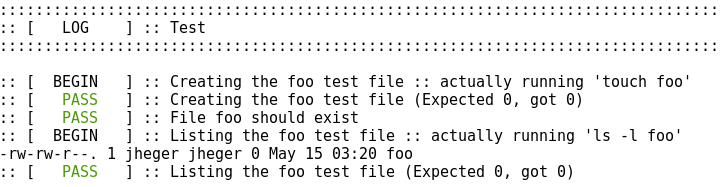
\includegraphics[width=\linewidth]{console_output.png}
  \caption{Snippet from console's output}
  \label{fig:console_output}
\end{figure}

\subsection{journal.xml}
Last output is a an XML\footnote{eXtensible Markup Language} file. This document is stripped off of executed commands' own output, but core information (such as which commands were executed, whether they passed or failed and so on) is kept. Also metadata about the test run (time of execution, which component was tested and more) as well as information about the hardware and software test was run on are added. \textit{journal.xml} is sent back to Beaker same as \textit{journal.txt} where it is available for further processing by automated tools. It also serves as a source of information about current state of the test during its execution, for example whether there is currently an open phase or how many failed tests or phases there are so far.

\section{Source files}
This section describes a few of BeakerLib's source files, relevant to this thesis.
\begin{itemize}
\item \textit{beakerlib.sh} - Starting point of every tests. It is \texttt{sourced} at the beginning of each test and in turn \texttt{sources} all other BeakerLib files.
\item \textit{testing.sh} - Contains definitions of the most used \textbf{rlCommands} as well as some internal functions.
\item \textit{journal.sh} - Provides bash-side Journaling functionality. Functions from this file process information about what to log and relay them to \textit{journalling.py}.
\item \textit{journalling.py} - Python script responsible for creating most of BeakerLib's outputs. It also creates and modifies \textit{journal.xml} file.
\end{itemize}

\section{Analysis of slow performance}
It was reported that BeakerLib suffers performance problems when running long tests. Time of processing each \textbf{rlCommand} grew longer after many (several hundreds and more) were used. Analysis of library was problematic due to lack of documentation, complex structure and uncommented code, however thorough investigation of the source code indicated that problem lies with generating \textit{journal.xml}. 

Python script \textit{journalling.py} is called after each \textbf{rlCommand} to log its result into \textit{journal.xml}. This isn't big problem with small test as the \textit{journal.xml} file takes up only a few kilobytes, however when the file takes up dozens or hundreds of kilobytes, repeated loading the file from disk, parsing, adding a line of log and then saving the file back to the disk adds significantly more load to CPU\footnote{Central Processing Unit}. Running larger tests therefore becomes quite time consuming and considerably slows down testing as a whole.

This has been determined as the main focus of the thesis since it probably is the most significant performance bottleneck. The next chapter describes proposed solutions with their pros and cons.

Figure \ref{fig:rl_run} illustrates simplified version of how \textbf{rlRun} propagates through different functions from BeakerLib files (which are \texttt{sourced} at the time test execution,  depicted by rounded rectangles) and how it is logged into the Journal. Similar operation is performed for every \textbf{rlCommand} in a test.

\begin{figure}[h!]
  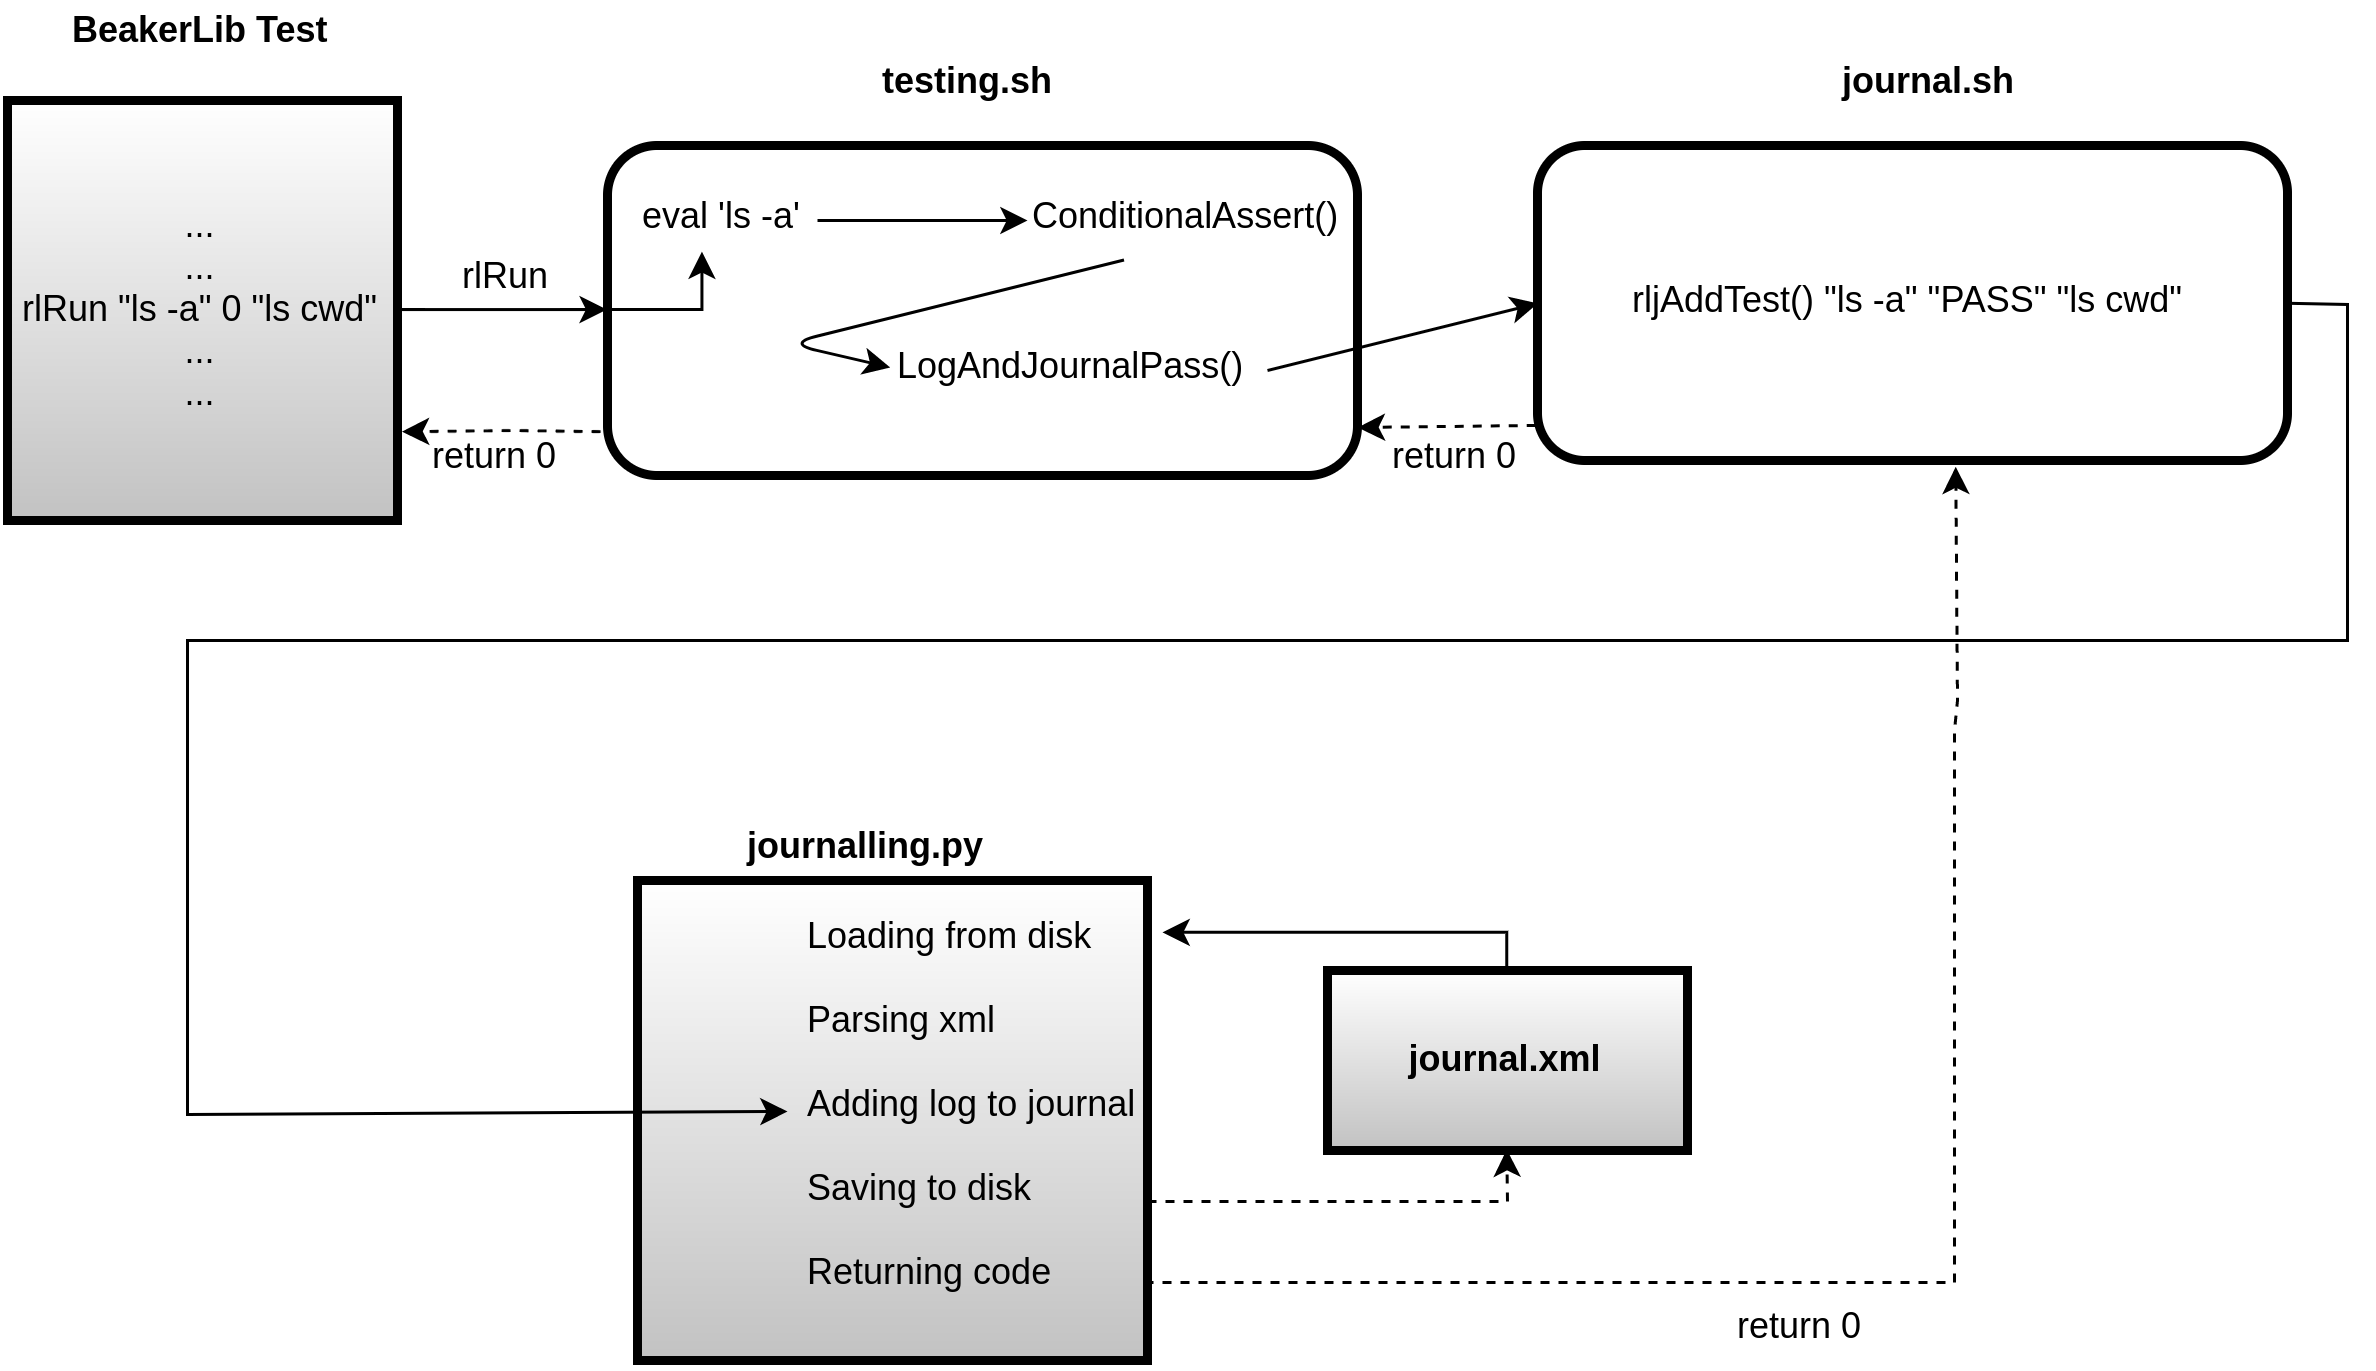
\includegraphics[width=\linewidth]{rl_run.png}
  \caption{Logging of rlRun to Journal}
  \label{fig:rl_run}
\end{figure}


\chapter{Solution of Journaling problem}
\label{solutions}

This chapter describes proposed solutions to optimize Journaling problem. Sections in this chapter provide possible solutions to the Journaling problem. Besides explaining the principle of each solution, the sections also discuss their advantages, disadvantages and potential issues.

\section{Change of xml parser}
XML parser is a program which can turn XML document into structured object in RAM\footnote{Random Access Memory}. Depending on implementation of the parser, that object is then easier to access by the program as it may provide methods to navigate the object and search it or potentially modify. 

Parsing of XML in BeakerLib is done by \textit{journalling.py} script by \texttt{Python} module \texttt{xml.dom.minidom}. 

 \texttt{xml.dom.minidom} is a native part of \texttt{Python} from version 2.0 and provides minimal implementation of the DOM\footnote{Document Object Model} interface, with an API\footnote{Application Programming Interface} similar to that in other languages. \cite{minidom_doc}

I decided to change parser to different one, to measure whether it will provide better performance. Because of reasons of backward compatibility with RHEL 5\footnote{Red Hat Enterprise Linux 5} which needs to be supported by BeakerLib, the choice of XML parsers was limited to native modules of \texttt{Python 2.4.3}. Two additional XML parsers were present for given version.

\begin{itemize}
\item lxml - The \texttt{lxml} XML toolkit is a Pythonic binding for the C libraries libxml2 and libxslt. It combines the speed and XML feature completeness of these libraries with the simplicity of a native \texttt{Python} API.  \cite{lxml_doc}

It works similarly to \texttt{xml.dom.minidom} in the way that when reading XML object from a file, it will read it whole, builds an object out of it and provides methods for the object to allow access to it.
\item xml.sax  \cite{sax_doc} - \texttt{xml.sax} originated as a parser for \texttt{Java}\cite{Sax2}. In \texttt{Python} it was released with version 2.0. It differs from \texttt{xml.dom.minidom} and \texttt{lxml} where the two mentioned parsers work with a whole XML file,  \texttt{xml.sax} emits events as it goes step by step through the file\cite{sax_example}. Using this approach means less memory has to be allocated for XML handling and therefore makes it ideal when working with very large amount of XML  data.
\end{itemize}

I decided to implement \texttt{lxml} parser as it is supposed to be faster and less demanding on memory than \texttt{xml.dom.minidom}\cite{lxml_performance}, while keeping its intuitive interface.

\section{Change in calling journalling.py}
Next proposition to make BeakerLib faster is in a way \textit{journalling.py} is called. The assumption being that repeated parsing of XML document slows BeakerLib the most, reducing the number of times it was parsed was then the highest priority. 

\subsection{Queue file solution}
First solution is to create a new, temporary \textbf{queue file}, which will act as a buffer. \textbf{rlCommands} will behave as before apart from creating BeakerLib journals but instead they will write message into the \textbf{queue file}. This file will be read and processed only when necessary, that is at the end each phase, when journals are sent to Beaker.

\subsubsection{Disadvantages}
The way BeakerLib is designed now it in most cases expects some form of return value from \textit{journalling.py} immediately after adding a log to a journal. Performed logging either returns code indicating success of failure or \texttt{string} with information about the current state of test. This presents problem as there is no way how to communicate back these information when parsing is postponed. 

\subsection{Daemon-like solution}
Second solution is to rewrite \textit{journalling.py} script to have daemon-like behavior. That is to have it run as its own process throughout the whole time of test execution. The XML object will be stored in memory, and parsed as whole only at the beginning of journal creation and in case of restarting the test run (which happen when machine is rebooted).  

This way BeakerLib can receive response about current test state immediately while still keeping CPU load minimal. Daemon-like solution however brings different obstacles.

\subsubsection{Disadvantages}
An independent, potentially long running process daemon is more prone to unplanned events such as unexpected exit. This must be addressed by both daemon (to exit as safely as possible)  and by the rest of BeakerLib (to detect that daemon is no longer running and to behave accordingly). 

\subsubsection{Communication}
Inter-process communication between running test and daemon has to be created for test to inform which \textbf{rlCommand} is supposed to be logged and for daemon to respond with current state of XML document. This two-way communication must be synchronous to assure BeakerLib and daemon process their respective messages in correct order. I considered following options:

\begin{itemize}
\item Unix sockets  -  <expand>
\item Named pipes - Named pipes are device files. They allow inter-process communication by reading it and writing into is as if regular file, however under normal circumstances the read/write is a blocking operation. This means if one process opens pipe for reading, it will hang there until another process opens the pipe for writing. This feature can be used for synchronization of communication between processes. 
\end{itemize}

% DOPLINT CITACE ^^ ???

I chose to implement communication through Named pipes because synchronization issue is taken care of because of the way Named pipes are designed.


\chapter{Implementation of proposed solutions}
\label{implementations}
This chapter describes how the proposed solutions were implemented. Each solution has its own section that describes implementation details and obstacles that were found and had to be solved during the implementation.
During changing of parsers I discovered and fixed few bugs present in current implementation of \textit{journalling.py}.

\section{Change of xml parser}
\subsection{Difference in parsers}
As mentioned before I chose to change original XML parser to \texttt{lxml}. Only changes in code were in file \textit{journalling.py} as it is only part of BeakerLib that directly works with journal's XML object. 
Most of the changes consisted in changing \texttt{xml.dom.minidom's} method for creating new XML element and assigning value into it.
Biggest difference between given parsers is that \texttt{lxml} does not provide many helping methods as \texttt{xml.dom.minidom} does.
For example in \texttt{lxml}  there is no method \texttt{getElementsByTagName()} to search XML object by a tag name. Instead \texttt{lxml} supports \texttt{xpath} \cite{xpath} syntax for searching the object. xpath\footnote{XML Path Language} is part of XSLT\footnote{eXtensible Stylesheet Language Transformations} standard. It be can used to navigate through elements and attributes in an XML document.

Another example of difference is an approach for accessing element's children. While \texttt{xml.dom.minidom} has dedicated methods and attributes such as \texttt{hasChildNodes()} which returns \texttt{bool} value or \texttt{childNodes} which is a iterable attribute of element's children, \texttt{lxml} has more low level implementation. It treats elements as python lists so \texttt{hasChildNodes()} can be replaced with simple \texttt{len(element) != 0}.
\\
\\
Because preliminary performance measurement showed faster test execution with \texttt{lxml}, I decided to implement the rest of the proposed solutions with this parser.

\section{Queue file solution}
This section deals with implementation of \textbf{queue file} solution. It is divided into subsections that discuss files I designed or changed during implementation. 

\subsection{Queue file}
\textbf{Queue file} was designed in a way so it was simple to implement, in a human readable format for potential test debugging and easy to extend by new, future functions that will work with it. 
It is a plain text file, each line containing one buffered command for \texttt{Python} script to process later, on demand. 

\subsection{journal.sh}
Creation of  \textbf{queue file}, by using \texttt{touch} command, was added to function \textbf{rlJournalStart()} which initializes Journaling functionality. It also \texttt{exports} new variable BEAKERLIB\_QUEUE, with \textbf{queue file's} path, into test's environment so \texttt{Python} script \textit{od\_journalling.py}, can later access it.

Original calling of \textit{journalling.py}, which is a main functionality of \textit{journal.sh}, was replaced in one of two ways:

\begin{itemize}
\item Delayed calling - New function \textbf{rljPrintToQueue()} takes all arguments that were originally meant for \textit{journalling.py} and instead prints them into \textbf{queue file}, where it will be processed by \textit{od\_journalling.py} later during execution of the test. This concerns functions which do not necessary require response about current test state from \textit{journal.xml}.  Namely functions: rlJournalPrint(), rljAddTest(), rljAddMetric(), rljAddMessage(), rljRpmLog()
\item Immediate calling of \textit{od\_journalling.py} - Virtually the same as the original solution. These functions require immediate response. Using this way of calling won't save on any CPU load (in fact the the load will be slightly higher than before because of operations related to \textbf{queue file} processing), however in typical BeakerLib test these functions are in minority compared to previous type of calling.  Functions and the response they require are:  
\begin{itemize}
\item rlJournalStart() - requires confirmation that journal was initiated successfully
\item rlJournalPrintText() - requires \textit{journal.txt} which is generated from current \mbox{\textit{journal.xml}}
\item rlGetTestState()  - requires number of failed asserts in the test so far
\item rlGetPhaseState() - requires number of failed phases in the test so far
\item rljAddPhase() - requires immediate print
\item rljClosePhase() - requires result of closed phase, to send it to Beaker along with Journal
\end{itemize}
\end{itemize}

Apart from printing to \textbf{queue file}, \textbf{rljPrintToQueue} also has to escape given arguments. This done because firstly some of the arguments originating from user may contain newline character which would break "one buffered command per line" rule in  \textbf{queue file} and secondly so \textit{od\_journalling.py} may parse it with \texttt{optparse} module.
Escaping is done with \texttt{printf} bash builtin\cite{bash_builtins}, specifically its \texttt{\%q} option which causes \texttt{printf} to output in \texttt{shell-quoted} format.

\subsection{od\_journalling.py}
File \textit{od\_journalling.py} originated from \textit{ournalling.py} but it differs in some ways.

Now when it is called, it first parses current \textit{journal.xml} and then calls new method \texttt{updateXML()} wtih parsed XML object as an argument. This method opens \textbf{queue file} and finds last line it accessed in previous call. From there it reads buffered lines and modifies the XML object accordingly.When it reaches end of file, it makes a mark for future readings and returns to the original call coming from \textit{journal.sh} 


\section{Daemon-like solution}

\section{testing that my solution is the same}

\chapter{Performance measuring}
\label{performance}
<Definition of performance measuring>

For performance measuring of BeakerLib I chose two kinds of tests in in two kinds of testing environments.

\section{Tests}

\subsection{Artificial tests}
First type of tests are artificial tests created by me with \texttt{beaker-wizard} tool to specifically target and measure performance of journaling modifications I made. They consist mostly of \textbf{rlCommands} that directly work with \texttt{journalling.py}. For example commands \textbf{rlLog} or \textbf{rlPhaseStart} and \textbf{rlPhaseEnd}. This way we can observe clear difference in performance without being affected by operations unrelated to journaling (executing actions that verify functionality of components in real tests). 

<description of artificial tests with links to Appendix>

\subsection{Real tests}
Second type are real tests used in Red Hat. These are examples of tests that have been reported to have bad performance with BeakerLib so I am testing them to see if my modifications have real life impact on performance.

<description of real tests>

\section{Testing Environment}

\subsection{Local}
First environment is local laptop for convenience and speed of execution. Tests were run directly, without any harness and with these technical specifications. 

<table of tech specs>

\subsection{Remote in beaker}
Second round of testing was done to emulate real testing conditions and to verify that changes made to BeakerLib do not break functionality outside of controlled environment. Tests were run with the default test harness Beah.
<table of tech specs>

\section{Measured Values}

\section{Baseline measurements}
<results>


\section{Implemented optimizations}
<results>

\chapter{Conclusion}
Recap of results
\\
Future work


%=========================================================================
